\documentclass[twoside]{book}

% Packages required by doxygen
\usepackage{fixltx2e}
\usepackage{calc}
\usepackage{doxygen}
\usepackage[export]{adjustbox} % also loads graphicx
\usepackage{graphicx}
\usepackage[utf8]{inputenc}
\usepackage{makeidx}
\usepackage{multicol}
\usepackage{multirow}
\PassOptionsToPackage{warn}{textcomp}
\usepackage{textcomp}
\usepackage[nointegrals]{wasysym}
\usepackage[table]{xcolor}

% Font selection
\usepackage[T1]{fontenc}
\usepackage[scaled=.90]{helvet}
\usepackage{courier}
\usepackage{amssymb}
\usepackage{sectsty}
\renewcommand{\familydefault}{\sfdefault}
\allsectionsfont{%
  \fontseries{bc}\selectfont%
  \color{darkgray}%
}
\renewcommand{\DoxyLabelFont}{%
  \fontseries{bc}\selectfont%
  \color{darkgray}%
}
\newcommand{\+}{\discretionary{\mbox{\scriptsize$\hookleftarrow$}}{}{}}

% Page & text layout
\usepackage{geometry}
\geometry{%
  a4paper,%
  top=2.5cm,%
  bottom=2.5cm,%
  left=2.5cm,%
  right=2.5cm%
}
\tolerance=750
\hfuzz=15pt
\hbadness=750
\setlength{\emergencystretch}{15pt}
\setlength{\parindent}{0cm}
\setlength{\parskip}{0.2cm}
\makeatletter
\renewcommand{\paragraph}{%
  \@startsection{paragraph}{4}{0ex}{-1.0ex}{1.0ex}{%
    \normalfont\normalsize\bfseries\SS@parafont%
  }%
}
\renewcommand{\subparagraph}{%
  \@startsection{subparagraph}{5}{0ex}{-1.0ex}{1.0ex}{%
    \normalfont\normalsize\bfseries\SS@subparafont%
  }%
}
\makeatother

% Headers & footers
\usepackage{fancyhdr}
\pagestyle{fancyplain}
\fancyhead[LE]{\fancyplain{}{\bfseries\thepage}}
\fancyhead[CE]{\fancyplain{}{}}
\fancyhead[RE]{\fancyplain{}{\bfseries\leftmark}}
\fancyhead[LO]{\fancyplain{}{\bfseries\rightmark}}
\fancyhead[CO]{\fancyplain{}{}}
\fancyhead[RO]{\fancyplain{}{\bfseries\thepage}}
\fancyfoot[LE]{\fancyplain{}{}}
\fancyfoot[CE]{\fancyplain{}{}}
\fancyfoot[RE]{\fancyplain{}{\bfseries\scriptsize Generated on Thu Apr 14 2016 23\+:58\+:32 for Practica4 by Doxygen }}
\fancyfoot[LO]{\fancyplain{}{\bfseries\scriptsize Generated on Thu Apr 14 2016 23\+:58\+:32 for Practica4 by Doxygen }}
\fancyfoot[CO]{\fancyplain{}{}}
\fancyfoot[RO]{\fancyplain{}{}}
\renewcommand{\footrulewidth}{0.4pt}
\renewcommand{\chaptermark}[1]{%
  \markboth{#1}{}%
}
\renewcommand{\sectionmark}[1]{%
  \markright{\thesection\ #1}%
}

% Indices & bibliography
\usepackage{natbib}
\usepackage[titles]{tocloft}
\setcounter{tocdepth}{3}
\setcounter{secnumdepth}{5}
\makeindex

% Hyperlinks (required, but should be loaded last)
\usepackage{ifpdf}
\ifpdf
  \usepackage[pdftex,pagebackref=true]{hyperref}
\else
  \usepackage[ps2pdf,pagebackref=true]{hyperref}
\fi
\hypersetup{%
  colorlinks=true,%
  linkcolor=blue,%
  citecolor=blue,%
  unicode%
}

% Custom commands
\newcommand{\clearemptydoublepage}{%
  \newpage{\pagestyle{empty}\cleardoublepage}%
}


%===== C O N T E N T S =====

\begin{document}

% Titlepage & ToC
\hypersetup{pageanchor=false,
             bookmarks=true,
             bookmarksnumbered=true,
             pdfencoding=unicode
            }
\pagenumbering{roman}
\begin{titlepage}
\vspace*{7cm}
\begin{center}%
{\Large Practica4 }\\
\vspace*{1cm}
{\large Generated by Doxygen 1.8.9.1}\\
\vspace*{0.5cm}
{\small Thu Apr 14 2016 23:58:32}\\
\end{center}
\end{titlepage}
\clearemptydoublepage
\tableofcontents
\clearemptydoublepage
\pagenumbering{arabic}
\hypersetup{pageanchor=true}

%--- Begin generated contents ---
\chapter{Hierarchical Index}
\section{Class Hierarchy}
This inheritance list is sorted roughly, but not completely, alphabetically\+:\begin{DoxyCompactList}
\item \contentsline{section}{Practica4.\+Arbitro}{\pageref{class_practica4_1_1_arbitro}}{}
\item \contentsline{section}{Practica4.\+Pelota}{\pageref{class_practica4_1_1_pelota}}{}
\item Runnable\begin{DoxyCompactList}
\item \contentsline{section}{Practica4.\+Jugador}{\pageref{class_practica4_1_1_jugador}}{}
\end{DoxyCompactList}
\end{DoxyCompactList}

\chapter{Class Index}
\section{Lista de clases}
Lista de las clases, estructuras, uniones e interfaces con una breve descripción\+:\begin{DoxyCompactList}
\item\contentsline{section}{\hyperlink{class_ejercicio1__3__3_1_1_detener___interrupcion}{Ejercicio1\+\_\+3\+\_\+3.\+Detener\+\_\+\+Interrupcion} \\*Thread que se detiene tras una señal del usuario, con diferentes acciones en función del tiempo transcurrido }{\pageref{class_ejercicio1__3__3_1_1_detener___interrupcion}}{}
\item\contentsline{section}{\hyperlink{class_ejercicio1__2__1_1_1_ejercicio1}{Ejercicio1\+\_\+2\+\_\+1.\+Ejercicio1} \\*Creación del número de hilos especificados por el usuario }{\pageref{class_ejercicio1__2__1_1_1_ejercicio1}}{}
\item\contentsline{section}{\hyperlink{class_ejercicio1__2__1_1_1_ejercicio2}{Ejercicio1\+\_\+2\+\_\+1.\+Ejercicio2} \\*Creación del número de hilos especificados por el usuario y medición del tiempo de ejecucion de los hilos }{\pageref{class_ejercicio1__2__1_1_1_ejercicio2}}{}
\item\contentsline{section}{\hyperlink{class_ejercicio1__2__4_1_1_ejercicio4}{Ejercicio1\+\_\+2\+\_\+4.\+Ejercicio4} \\*Cada thread calcula su tiempo de ejecución, lo almacena en una variable publica y se calcula el tiempo total }{\pageref{class_ejercicio1__2__4_1_1_ejercicio4}}{}
\item\contentsline{section}{\hyperlink{class_ejercicio1__2__5_1_1_ejercicio5}{Ejercicio1\+\_\+2\+\_\+5.\+Ejercicio5} \\*Muestra por separados los tiempos de inicialización de threads y los tiempos de ejecución de threads }{\pageref{class_ejercicio1__2__5_1_1_ejercicio5}}{}
\item\contentsline{section}{\hyperlink{class_ejercicio1__2__6_1_1_ejercicio6}{Ejercicio1\+\_\+2\+\_\+6.\+Ejercicio6} \\*Al crear los threads, en caso de introducir el valor \char`\"{}1\char`\"{} se realiza una operación compleja, en caso contrario se procede a la identificación finalización de los threads }{\pageref{class_ejercicio1__2__6_1_1_ejercicio6}}{}
\item\contentsline{section}{\hyperlink{class_ejercicio1__1__2_1_1hello_runnable}{Ejercicio1\+\_\+1\+\_\+2.\+hello\+Runnable} \\*Creación de hilos usando la clase Runnable }{\pageref{class_ejercicio1__1__2_1_1hello_runnable}}{}
\item\contentsline{section}{\hyperlink{class_ejercicio1__1__3_1_1hello_runnable___sleep}{Ejercicio1\+\_\+1\+\_\+3.\+hello\+Runnable\+\_\+\+Sleep} \\*Creación de hilos usando la clase Runnable y usando el método sleep para crear el delay de 1 segundo }{\pageref{class_ejercicio1__1__3_1_1hello_runnable___sleep}}{}
\item\contentsline{section}{\hyperlink{class_ejercicio1__1__2_1_1hello_thread}{Ejercicio1\+\_\+1\+\_\+2.\+hello\+Thread} \\*Creación de hilos usando la clase Thread }{\pageref{class_ejercicio1__1__2_1_1hello_thread}}{}
\item\contentsline{section}{\hyperlink{class_ejercicio1__1__3_1_1hello_thread___sleep}{Ejercicio1\+\_\+1\+\_\+3.\+hello\+Thread\+\_\+\+Sleep} \\*Creación de hilos usando la clase Thread y usando el método sleep para crear el delay de 1 segundo }{\pageref{class_ejercicio1__1__3_1_1hello_thread___sleep}}{}
\item\contentsline{section}{\hyperlink{class_ejercicio1__1__4_1_1_runnable___activo}{Ejercicio1\+\_\+1\+\_\+4.\+Runnable\+\_\+\+Activo} \\*Creación de hilos usando la clase Runnable y usando los metodos active\+Count y current\+Thread para postrar el numero de hilos y el hilo actual }{\pageref{class_ejercicio1__1__4_1_1_runnable___activo}}{}
\item\contentsline{section}{\hyperlink{class_ejercicio1__1__4_1_1_thread___activo}{Ejercicio1\+\_\+1\+\_\+4.\+Thread\+\_\+\+Activo} \\*Creación de hilos usando la clase Thread y usando los metodos active\+Count y current\+Thread para postrar el numero de hilos y el hilo actual }{\pageref{class_ejercicio1__1__4_1_1_thread___activo}}{}
\item\contentsline{section}{\hyperlink{class_ejercicio1__3__2_1_1_thread___detenido}{Ejercicio1\+\_\+3\+\_\+2.\+Thread\+\_\+\+Detenido} \\*Crea un Thread y comprueba con is\+Interrupted() e interrupted() antes y después de interrumpirlo }{\pageref{class_ejercicio1__3__2_1_1_thread___detenido}}{}
\end{DoxyCompactList}

\chapter{Class Documentation}
\hypertarget{class_practica4_1_1_arbitro}{}\section{Practica4.\+Arbitro Class Reference}
\label{class_practica4_1_1_arbitro}\index{Practica4.\+Arbitro@{Practica4.\+Arbitro}}


Clase main, que decide quién comienza jugando, cuántos turnos, modo de juego e inicia el juego.  


\subsection*{Static Public Member Functions}
\begin{DoxyCompactItemize}
\item 
\hypertarget{class_practica4_1_1_arbitro_ab357066d6d94d3daedb4d19b13111f17}{}static void {\bfseries main} (String\mbox{[}$\,$\mbox{]} args)\label{class_practica4_1_1_arbitro_ab357066d6d94d3daedb4d19b13111f17}

\end{DoxyCompactItemize}


\subsection{Detailed Description}
Clase main, que decide quién comienza jugando, cuántos turnos, modo de juego e inicia el juego. 

\begin{DoxyAuthor}{Author}
Nara, Javier, Esteban 
\end{DoxyAuthor}


The documentation for this class was generated from the following file\+:\begin{DoxyCompactItemize}
\item 
Arbitro.\+java\end{DoxyCompactItemize}

\hypertarget{class_practica4_1_1_jugador}{}\section{Practica4.\+Jugador Class Reference}
\label{class_practica4_1_1_jugador}\index{Practica4.\+Jugador@{Practica4.\+Jugador}}


Clase que implementa los threads del Ping Pong.  




Inheritance diagram for Practica4.\+Jugador\+:
\nopagebreak
\begin{figure}[H]
\begin{center}
\leavevmode
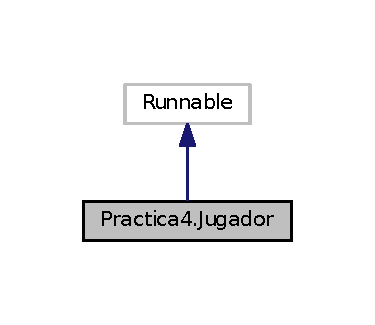
\includegraphics[width=180pt]{class_practica4_1_1_jugador__inherit__graph}
\end{center}
\end{figure}


Collaboration diagram for Practica4.\+Jugador\+:
\nopagebreak
\begin{figure}[H]
\begin{center}
\leavevmode
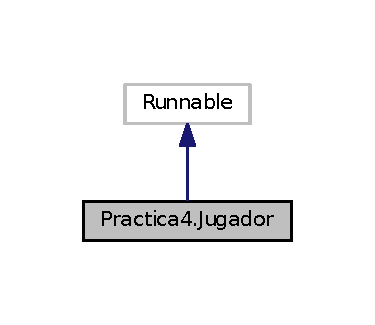
\includegraphics[width=180pt]{class_practica4_1_1_jugador__coll__graph}
\end{center}
\end{figure}
\subsection*{Public Member Functions}
\begin{DoxyCompactItemize}
\item 
\hyperlink{class_practica4_1_1_jugador_aee0431507107aa41280193b75e396437}{Jugador} (int id, \hyperlink{class_practica4_1_1_pelota}{Pelota} pelota)
\begin{DoxyCompactList}\small\item\em Método constructor de la clase. \end{DoxyCompactList}\item 
void \hyperlink{class_practica4_1_1_jugador_a95fb1e508af2d77aee30222cb64199c2}{run} ()
\begin{DoxyCompactList}\small\item\em Método run en el que se realzará ping o pong si es el turno del el Thread en ejecución y se desbloquearán todos los threads en caso contrario, se bloqueará el thread. \end{DoxyCompactList}\end{DoxyCompactItemize}


\subsection{Detailed Description}
Clase que implementa los threads del Ping Pong. 

\begin{DoxyAuthor}{Author}
Nara, Javier, Esteban 
\end{DoxyAuthor}


\subsection{Constructor \& Destructor Documentation}
\hypertarget{class_practica4_1_1_jugador_aee0431507107aa41280193b75e396437}{}\index{Practica4\+::\+Jugador@{Practica4\+::\+Jugador}!Jugador@{Jugador}}
\index{Jugador@{Jugador}!Practica4\+::\+Jugador@{Practica4\+::\+Jugador}}
\subsubsection[{Jugador}]{\setlength{\rightskip}{0pt plus 5cm}Practica4.\+Jugador.\+Jugador (
\begin{DoxyParamCaption}
\item[{int}]{id, }
\item[{{\bf Pelota}}]{pelota}
\end{DoxyParamCaption}
)}\label{class_practica4_1_1_jugador_aee0431507107aa41280193b75e396437}


Método constructor de la clase. 

\begin{DoxyAuthor}{Author}
Nara, Javier, Esteban 
\end{DoxyAuthor}

\begin{DoxyParams}{Parameters}
{\em id} & \+: Número identificador del jugador a crear \\
\hline
{\em pelota} & \+: Objeto pelota con la cual se realizará el juego \\
\hline
\end{DoxyParams}


\subsection{Member Function Documentation}
\hypertarget{class_practica4_1_1_jugador_a95fb1e508af2d77aee30222cb64199c2}{}\index{Practica4\+::\+Jugador@{Practica4\+::\+Jugador}!run@{run}}
\index{run@{run}!Practica4\+::\+Jugador@{Practica4\+::\+Jugador}}
\subsubsection[{run}]{\setlength{\rightskip}{0pt plus 5cm}void Practica4.\+Jugador.\+run (
\begin{DoxyParamCaption}
{}
\end{DoxyParamCaption}
)}\label{class_practica4_1_1_jugador_a95fb1e508af2d77aee30222cb64199c2}


Método run en el que se realzará ping o pong si es el turno del el Thread en ejecución y se desbloquearán todos los threads en caso contrario, se bloqueará el thread. 

\begin{DoxyAuthor}{Author}
Nara, Javier, Esteban 
\end{DoxyAuthor}


The documentation for this class was generated from the following file\+:\begin{DoxyCompactItemize}
\item 
Jugador.\+java\end{DoxyCompactItemize}

\hypertarget{class_practica4_1_1_pelota}{}\section{Practica4.\+Pelota Class Reference}
\label{class_practica4_1_1_pelota}\index{Practica4.\+Pelota@{Practica4.\+Pelota}}


Clase que implementa el objeto \hyperlink{class_practica4_1_1_pelota}{Pelota} para permitir jugar al Ping Pong.  


\subsection*{Public Member Functions}
\begin{DoxyCompactItemize}
\item 
\hyperlink{class_practica4_1_1_pelota_a9bba2cb1e5adaf75e6f994d1e888c510}{Pelota} (int turno, int jugadores, int max\+Jugadas, int modalidad)
\begin{DoxyCompactList}\small\item\em Método constructor de la clase. \end{DoxyCompactList}\item 
void \hyperlink{class_practica4_1_1_pelota_ab11c5110d330f07f4ae8c6db9a4ffc10}{set\+Turno} (int turno)
\begin{DoxyCompactList}\small\item\em Método que asinga el jugador al cuál le corresponde el turno. \end{DoxyCompactList}\item 
int \hyperlink{class_practica4_1_1_pelota_a188f4792d7cba45b3ccd838712f2da45}{get\+Turno} ()
\begin{DoxyCompactList}\small\item\em Método que obtiene el jugador al cuál le corresponde el turno. \end{DoxyCompactList}\item 
void \hyperlink{class_practica4_1_1_pelota_a7a63bb6a91aa761d199bf4f52121929c}{set\+Estado} (boolean bool)
\begin{DoxyCompactList}\small\item\em Método que cambia el estado del juego (termina el juego) \end{DoxyCompactList}\item 
boolean \hyperlink{class_practica4_1_1_pelota_ac35ca764f2c6e26db922a6f5c726fc18}{get\+Estado} ()
\begin{DoxyCompactList}\small\item\em Método que obtiene el estado del juego (termina el juego) \end{DoxyCompactList}\item 
int \hyperlink{class_practica4_1_1_pelota_a1149eb47d7a21c21710d00e5c223e527}{get\+Jugadores} ()
\begin{DoxyCompactList}\small\item\em Método que obtiene cuántos jugadores hay en el partido. \end{DoxyCompactList}\item 
int \hyperlink{class_practica4_1_1_pelota_ad72f2a2d2a0b26f3b19ace9ed6cf65d3}{get\+Jugadas} ()
\begin{DoxyCompactList}\small\item\em Método que obtiene cuántos turnos se han realozado. \end{DoxyCompactList}\item 
void \hyperlink{class_practica4_1_1_pelota_add2d52594c65fce854d719668d923721}{incrementar\+Jugada} ()
\begin{DoxyCompactList}\small\item\em Método que incrementa en 1 el número de turnos que se han realozado. \end{DoxyCompactList}\item 
int \hyperlink{class_practica4_1_1_pelota_ad9423a6e3d425befd4c6809f0a7739a3}{get\+Max\+Jugadas} ()
\begin{DoxyCompactList}\small\item\em Método que obtiene cuántos turnos se deben realizar en el partido. \end{DoxyCompactList}\item 
int \hyperlink{class_practica4_1_1_pelota_aee2a61575064881875d6bcfc836f4fa9}{get\+Modalidad} ()
\begin{DoxyCompactList}\small\item\em Método que obtiene cómo se llevará a cabo el partido (por tiempo o por turnos) \end{DoxyCompactList}\item 
void \hyperlink{class_practica4_1_1_pelota_aca64e664ed97d572b2965dad0f3a6b7c}{set\+Texto} (boolean texto)
\begin{DoxyCompactList}\small\item\em Método que asigna qué texto debe salir por pantalla (ping o pong) \end{DoxyCompactList}\item 
boolean \hyperlink{class_practica4_1_1_pelota_ac45780f814a1c62684087f68a18b6f1e}{get\+Texto} ()
\begin{DoxyCompactList}\small\item\em Método que obtiene qué texto debe salir por pantalla (ping o pong) \end{DoxyCompactList}\end{DoxyCompactItemize}


\subsection{Detailed Description}
Clase que implementa el objeto \hyperlink{class_practica4_1_1_pelota}{Pelota} para permitir jugar al Ping Pong. 

\begin{DoxyAuthor}{Author}
Nara, Javier, Esteban 
\end{DoxyAuthor}


\subsection{Constructor \& Destructor Documentation}
\hypertarget{class_practica4_1_1_pelota_a9bba2cb1e5adaf75e6f994d1e888c510}{}\index{Practica4\+::\+Pelota@{Practica4\+::\+Pelota}!Pelota@{Pelota}}
\index{Pelota@{Pelota}!Practica4\+::\+Pelota@{Practica4\+::\+Pelota}}
\subsubsection[{Pelota}]{\setlength{\rightskip}{0pt plus 5cm}Practica4.\+Pelota.\+Pelota (
\begin{DoxyParamCaption}
\item[{int}]{turno, }
\item[{int}]{jugadores, }
\item[{int}]{max\+Jugadas, }
\item[{int}]{modalidad}
\end{DoxyParamCaption}
)}\label{class_practica4_1_1_pelota_a9bba2cb1e5adaf75e6f994d1e888c510}


Método constructor de la clase. 

\begin{DoxyAuthor}{Author}
Nara, Javier, Esteban 
\end{DoxyAuthor}

\begin{DoxyParams}{Parameters}
{\em turno} & \+: Número del jugador al que le toca jugar \\
\hline
{\em jugadores} & \+: Número de jugadores del partido \\
\hline
{\em max\+Jugadas} & \+: Número de turnos que se realizarán en el juego \\
\hline
{\em modalidad} & \+: Identificador que indica si el juego será por turnos o por tiempo \\
\hline
\end{DoxyParams}


\subsection{Member Function Documentation}
\hypertarget{class_practica4_1_1_pelota_ac35ca764f2c6e26db922a6f5c726fc18}{}\index{Practica4\+::\+Pelota@{Practica4\+::\+Pelota}!get\+Estado@{get\+Estado}}
\index{get\+Estado@{get\+Estado}!Practica4\+::\+Pelota@{Practica4\+::\+Pelota}}
\subsubsection[{get\+Estado}]{\setlength{\rightskip}{0pt plus 5cm}boolean Practica4.\+Pelota.\+get\+Estado (
\begin{DoxyParamCaption}
{}
\end{DoxyParamCaption}
)}\label{class_practica4_1_1_pelota_ac35ca764f2c6e26db922a6f5c726fc18}


Método que obtiene el estado del juego (termina el juego) 

\begin{DoxyAuthor}{Author}
Nara, Javier, Esteban 
\end{DoxyAuthor}
\begin{DoxyReturn}{Returns}
int estado \+: Estado que tendrá el juego 
\end{DoxyReturn}
\hypertarget{class_practica4_1_1_pelota_ad72f2a2d2a0b26f3b19ace9ed6cf65d3}{}\index{Practica4\+::\+Pelota@{Practica4\+::\+Pelota}!get\+Jugadas@{get\+Jugadas}}
\index{get\+Jugadas@{get\+Jugadas}!Practica4\+::\+Pelota@{Practica4\+::\+Pelota}}
\subsubsection[{get\+Jugadas}]{\setlength{\rightskip}{0pt plus 5cm}int Practica4.\+Pelota.\+get\+Jugadas (
\begin{DoxyParamCaption}
{}
\end{DoxyParamCaption}
)}\label{class_practica4_1_1_pelota_ad72f2a2d2a0b26f3b19ace9ed6cf65d3}


Método que obtiene cuántos turnos se han realozado. 

\begin{DoxyAuthor}{Author}
Nara, Javier, Esteban 
\end{DoxyAuthor}
\begin{DoxyReturn}{Returns}
jugadas \+: Número de turnos que se han realizado 
\end{DoxyReturn}
\hypertarget{class_practica4_1_1_pelota_a1149eb47d7a21c21710d00e5c223e527}{}\index{Practica4\+::\+Pelota@{Practica4\+::\+Pelota}!get\+Jugadores@{get\+Jugadores}}
\index{get\+Jugadores@{get\+Jugadores}!Practica4\+::\+Pelota@{Practica4\+::\+Pelota}}
\subsubsection[{get\+Jugadores}]{\setlength{\rightskip}{0pt plus 5cm}int Practica4.\+Pelota.\+get\+Jugadores (
\begin{DoxyParamCaption}
{}
\end{DoxyParamCaption}
)}\label{class_practica4_1_1_pelota_a1149eb47d7a21c21710d00e5c223e527}


Método que obtiene cuántos jugadores hay en el partido. 

\begin{DoxyAuthor}{Author}
Nara, Javier, Esteban 
\end{DoxyAuthor}
\begin{DoxyReturn}{Returns}
jugadores \+: Número de jugadores del partido 
\end{DoxyReturn}
\hypertarget{class_practica4_1_1_pelota_ad9423a6e3d425befd4c6809f0a7739a3}{}\index{Practica4\+::\+Pelota@{Practica4\+::\+Pelota}!get\+Max\+Jugadas@{get\+Max\+Jugadas}}
\index{get\+Max\+Jugadas@{get\+Max\+Jugadas}!Practica4\+::\+Pelota@{Practica4\+::\+Pelota}}
\subsubsection[{get\+Max\+Jugadas}]{\setlength{\rightskip}{0pt plus 5cm}int Practica4.\+Pelota.\+get\+Max\+Jugadas (
\begin{DoxyParamCaption}
{}
\end{DoxyParamCaption}
)}\label{class_practica4_1_1_pelota_ad9423a6e3d425befd4c6809f0a7739a3}


Método que obtiene cuántos turnos se deben realizar en el partido. 

\begin{DoxyAuthor}{Author}
Nara, Javier, Esteban 
\end{DoxyAuthor}
\begin{DoxyReturn}{Returns}
max\+Jugadas \+: Número de turnos que se deben realizar 
\end{DoxyReturn}
\hypertarget{class_practica4_1_1_pelota_aee2a61575064881875d6bcfc836f4fa9}{}\index{Practica4\+::\+Pelota@{Practica4\+::\+Pelota}!get\+Modalidad@{get\+Modalidad}}
\index{get\+Modalidad@{get\+Modalidad}!Practica4\+::\+Pelota@{Practica4\+::\+Pelota}}
\subsubsection[{get\+Modalidad}]{\setlength{\rightskip}{0pt plus 5cm}int Practica4.\+Pelota.\+get\+Modalidad (
\begin{DoxyParamCaption}
{}
\end{DoxyParamCaption}
)}\label{class_practica4_1_1_pelota_aee2a61575064881875d6bcfc836f4fa9}


Método que obtiene cómo se llevará a cabo el partido (por tiempo o por turnos) 

\begin{DoxyAuthor}{Author}
Nara, Javier, Esteban 
\end{DoxyAuthor}
\begin{DoxyReturn}{Returns}
modalidad \+: Modalidad que se jugará 
\end{DoxyReturn}
\hypertarget{class_practica4_1_1_pelota_ac45780f814a1c62684087f68a18b6f1e}{}\index{Practica4\+::\+Pelota@{Practica4\+::\+Pelota}!get\+Texto@{get\+Texto}}
\index{get\+Texto@{get\+Texto}!Practica4\+::\+Pelota@{Practica4\+::\+Pelota}}
\subsubsection[{get\+Texto}]{\setlength{\rightskip}{0pt plus 5cm}boolean Practica4.\+Pelota.\+get\+Texto (
\begin{DoxyParamCaption}
{}
\end{DoxyParamCaption}
)}\label{class_practica4_1_1_pelota_ac45780f814a1c62684087f68a18b6f1e}


Método que obtiene qué texto debe salir por pantalla (ping o pong) 

\begin{DoxyAuthor}{Author}
Nara, Javier, Esteban 
\end{DoxyAuthor}
\begin{DoxyReturn}{Returns}
texto \+: Valor que identifica qué texto saldrá por pantalla 
\end{DoxyReturn}
\hypertarget{class_practica4_1_1_pelota_a188f4792d7cba45b3ccd838712f2da45}{}\index{Practica4\+::\+Pelota@{Practica4\+::\+Pelota}!get\+Turno@{get\+Turno}}
\index{get\+Turno@{get\+Turno}!Practica4\+::\+Pelota@{Practica4\+::\+Pelota}}
\subsubsection[{get\+Turno}]{\setlength{\rightskip}{0pt plus 5cm}int Practica4.\+Pelota.\+get\+Turno (
\begin{DoxyParamCaption}
{}
\end{DoxyParamCaption}
)}\label{class_practica4_1_1_pelota_a188f4792d7cba45b3ccd838712f2da45}


Método que obtiene el jugador al cuál le corresponde el turno. 

\begin{DoxyAuthor}{Author}
Nara, Javier, Esteban 
\end{DoxyAuthor}
\begin{DoxyReturn}{Returns}
turno \+: Número del jugador al que le toca jugar 
\end{DoxyReturn}
\hypertarget{class_practica4_1_1_pelota_add2d52594c65fce854d719668d923721}{}\index{Practica4\+::\+Pelota@{Practica4\+::\+Pelota}!incrementar\+Jugada@{incrementar\+Jugada}}
\index{incrementar\+Jugada@{incrementar\+Jugada}!Practica4\+::\+Pelota@{Practica4\+::\+Pelota}}
\subsubsection[{incrementar\+Jugada}]{\setlength{\rightskip}{0pt plus 5cm}void Practica4.\+Pelota.\+incrementar\+Jugada (
\begin{DoxyParamCaption}
{}
\end{DoxyParamCaption}
)}\label{class_practica4_1_1_pelota_add2d52594c65fce854d719668d923721}


Método que incrementa en 1 el número de turnos que se han realozado. 

\begin{DoxyAuthor}{Author}
Nara, Javier, Esteban 
\end{DoxyAuthor}
\hypertarget{class_practica4_1_1_pelota_a7a63bb6a91aa761d199bf4f52121929c}{}\index{Practica4\+::\+Pelota@{Practica4\+::\+Pelota}!set\+Estado@{set\+Estado}}
\index{set\+Estado@{set\+Estado}!Practica4\+::\+Pelota@{Practica4\+::\+Pelota}}
\subsubsection[{set\+Estado}]{\setlength{\rightskip}{0pt plus 5cm}void Practica4.\+Pelota.\+set\+Estado (
\begin{DoxyParamCaption}
\item[{boolean}]{bool}
\end{DoxyParamCaption}
)}\label{class_practica4_1_1_pelota_a7a63bb6a91aa761d199bf4f52121929c}


Método que cambia el estado del juego (termina el juego) 

\begin{DoxyAuthor}{Author}
Nara, Javier, Esteban 
\end{DoxyAuthor}

\begin{DoxyParams}{Parameters}
{\em bool} & \+: Estado que tendrá el juego \\
\hline
\end{DoxyParams}
\hypertarget{class_practica4_1_1_pelota_aca64e664ed97d572b2965dad0f3a6b7c}{}\index{Practica4\+::\+Pelota@{Practica4\+::\+Pelota}!set\+Texto@{set\+Texto}}
\index{set\+Texto@{set\+Texto}!Practica4\+::\+Pelota@{Practica4\+::\+Pelota}}
\subsubsection[{set\+Texto}]{\setlength{\rightskip}{0pt plus 5cm}void Practica4.\+Pelota.\+set\+Texto (
\begin{DoxyParamCaption}
\item[{boolean}]{texto}
\end{DoxyParamCaption}
)}\label{class_practica4_1_1_pelota_aca64e664ed97d572b2965dad0f3a6b7c}


Método que asigna qué texto debe salir por pantalla (ping o pong) 

\begin{DoxyAuthor}{Author}
Nara, Javier, Esteban 
\end{DoxyAuthor}
\hypertarget{class_practica4_1_1_pelota_ab11c5110d330f07f4ae8c6db9a4ffc10}{}\index{Practica4\+::\+Pelota@{Practica4\+::\+Pelota}!set\+Turno@{set\+Turno}}
\index{set\+Turno@{set\+Turno}!Practica4\+::\+Pelota@{Practica4\+::\+Pelota}}
\subsubsection[{set\+Turno}]{\setlength{\rightskip}{0pt plus 5cm}void Practica4.\+Pelota.\+set\+Turno (
\begin{DoxyParamCaption}
\item[{int}]{turno}
\end{DoxyParamCaption}
)}\label{class_practica4_1_1_pelota_ab11c5110d330f07f4ae8c6db9a4ffc10}


Método que asinga el jugador al cuál le corresponde el turno. 

\begin{DoxyAuthor}{Author}
Nara, Javier, Esteban 
\end{DoxyAuthor}

\begin{DoxyParams}{Parameters}
{\em turno} & \+: Número del jugador al que le toca jugar \\
\hline
\end{DoxyParams}


The documentation for this class was generated from the following file\+:\begin{DoxyCompactItemize}
\item 
Pelota.\+java\end{DoxyCompactItemize}

%--- End generated contents ---

% Index
\backmatter
\newpage
\phantomsection
\clearemptydoublepage
\addcontentsline{toc}{chapter}{Index}
\printindex

\end{document}
